\subsection{Overview}
The system to be designed needs to help customers make reservations in their favourite shops in the least amount of time possible and also keep track of all the future appointments they have taken.\\
It also must allow shop owners to register their establishment to the platform and keep track of the next customers that have registered an appointment.\\
Since this interaction between user and system can be summarize as:
\begin{enumerate}
	\item User request a service to the system.
	\item System responds to the user with the requested service.
\end{enumerate}
Based on this, a client-server architectural approach has been chosen.
\begin{figure}[H]
	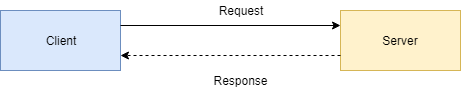
\includegraphics{Img/ClientServerArchitecture}
	\caption{Client Server architecture}
	\label{fig:clientserver}
\end{figure}
Furthermore, the system can be divided into three different subsystems: the presentation layer, the application layer and the data layer, where: 
\begin{itemize}
	\item The \emph{Presentation Layer} provides the GUI of the system.
	\item The \emph{Logic Layer} contains the logic of the application,that receives the requests from the user.
	\item The \emph{Data Layer} stores and maintains the data needed from the system to works properly, i.e. user's \& shop's information and reservations details.
\end{itemize}
\clearpage

\subsection{Component View}

\subsubsection{Overview}
In \autoref{fig:hlCD} is possible to see the high level components of the system and the interfaces used to connect one to another, where
\begin{itemize}
	\item \emph{Firebase} provides the entry point for external resources;
		\item \emph{Firestore} provides the database system;
			\item \emph{Firebase Auth} provides the authentication system;
	\item the \emph{Mobile Application} is the mobile application used by a user with his/her smartphone.
\end{itemize}

\begin{figure}[H]
	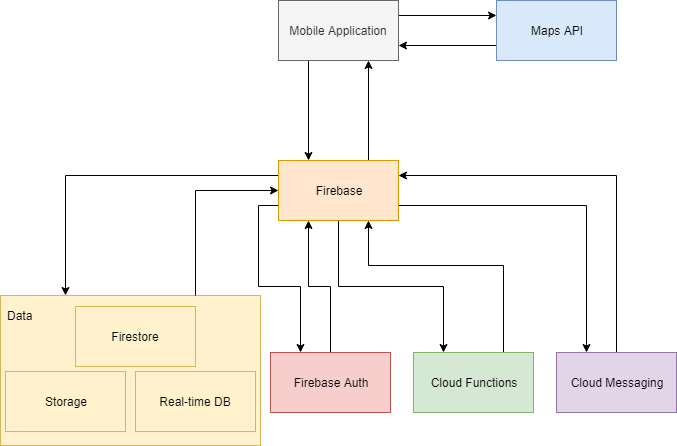
\includegraphics[width = \textwidth, keepaspectratio = true]{Img/HighLevelComponent}
	\caption{High level Component Diagram}
	\label{fig:hlCD}
\end{figure}

\clearpage
\subsubsection{Database View}
Unlike traditional Entity-Relationship DB systems, Firestore is organized in Collections-Documents hierarchy that can be further nested, meaning a Document can contain one or more Collections containing other Documents and so on.\\
For this project only three Collections where used, each composed by a series of documents as shown in \autoref{fig:HighLevelDB}
\begin{figure}[H]
	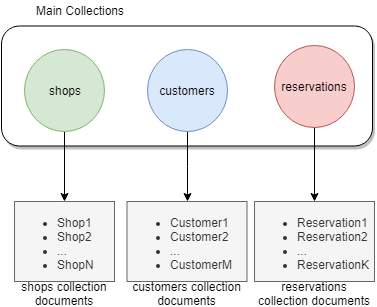
\includegraphics[width = 0.8\textwidth, keepaspectratio = true]{Img/HighLevelDB}
	\caption{\emph{High level} structure of the DB}
	\label{fig:HighLevelDB}
\end{figure}
\clearpage
\noindent While the three documents are shown as follows as a Java class would be. Shop \autoref{fig:ShopDocument} and Customer \autoref{fig:CustomerDocument} are actually implemented in this way, while reservations \autoref{fig:ReservationDocument} differ depending on the type of user that is using the application, but only these information are needed to be recorded in the database.
\begin{figure}[H]
  \centering
  \begin{minipage}[b]{0.3\textwidth}
    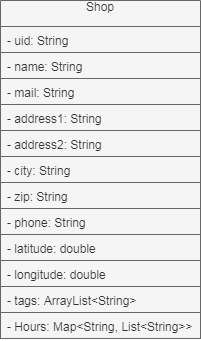
\includegraphics[width=\textwidth]{Img/ShopDocument}
	\caption{\emph{Shop} document}
	  \label{fig:ShopDocument}
  \end{minipage}
  \hfill
  \begin{minipage}[b]{0.3\textwidth}
    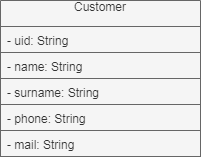
\includegraphics[width=\textwidth]{Img/CustomerDocument}
	\caption{\emph{Customer} document}
	  \label{fig:CustomerDocument}
  \end{minipage}
  \hfill
  \begin{minipage}[b]{0.3\textwidth}
    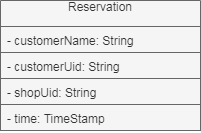
\includegraphics[width=\textwidth]{Img/ReservationDocument}
	\caption{\emph{Reservation} document}
	  \label{fig:ReservationDocument}
  \end{minipage}
\end{figure}

\subsubsection{Firebase Auth View}
The Firebase Authentication system handles automatically the authentication of the connected user by storing:
\begin{itemize}
\item Identifier (for example email address)
\item Provider (Email/Gmail account/Phone etc...)
\item Creation date
\item Last sign in
\item User UID (which is then used in the DB as an identifier)
\end{itemize} 
\subsubsection{Mobile Application}
The \emph{Mobile Application} is used by the user via its own smart device. The \emph{Mobile Application} communicates directly with the Firebase system using the provided API.
\clearpage

\subsection{Implementation choices}
\label{Implementation choices}
The technology chosen for the implementation on the system are all based on Java since it is the most common way of developing Android applications and the availability of documentation and other sources of learning materials are abundant and some experience was already obtained during past projects. It also offers the possibility of adding new functionalities in future, making the system more scalable given how the platform is constantly evolving\\
To summarize the technologies used:
\paragraph{Mobile application}: entirely Android (Java) based with Firebase API added in order to use the external tools. Other modules such as RecycleViews and Cards have been added.
\paragraph{DBMS}: Firestore was selected over the old real time database system since it has been developed as a successor to substitute it. I provides easy to use DB mechanisms, at the loss of complexity such as complex queries and it's not a relational DB system which is usually more familiar.\\

\clearpage
\subsection{Runtime View}
Here are represented the two most important runtime views by using diagrams that highlight the main actions the user has to follow in order to complete the given task.\\
In \autoref{fig:RegistrationDiagram} it's highlighted in red the interaction that the system has with the authentication system, then the two branches between choosing to register as a customer (green) or shop (blue) are available to be picked.\\
In \autoref{fig:ReservationDiagram} are again highlighted in red the interactions of the application with the Firebase systems, while in blue is noted the optional choice to select a different distance than the default one.\\
It should be noted how in both cases none of the handled errors or problems are shown to keep the diagrams simple.

\begin{figure}[H]
  \centering
  \begin{minipage}[b]{0.45\textwidth}
    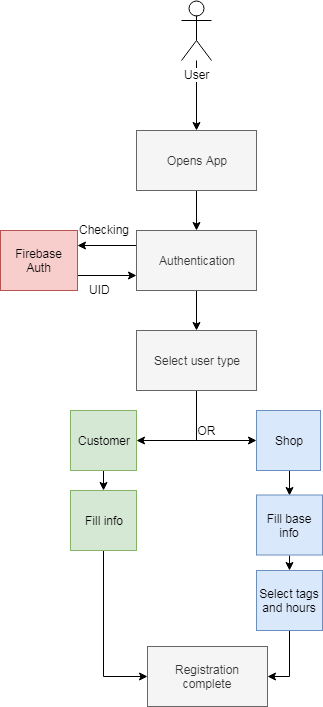
\includegraphics[width=\textwidth]{Img/RegistrationDiagram}
	\caption{\emph{User} registration diagram}
	  \label{fig:RegistrationDiagram}
  \end{minipage}
  \hfill
  \begin{minipage}[b]{0.45\textwidth}
    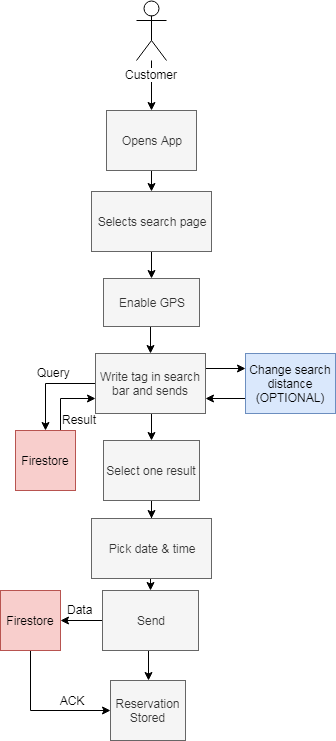
\includegraphics[width=\textwidth]{Img/ReservationDiagram}
	\caption{\emph{Customer} reservation process}
	  \label{fig:ReservationDiagram}
  \end{minipage}
\end{figure}














